In order to evaluate the proposed algorithms, the following metrics were considered:
\begin{inlinelist}
	\item Total reward;
	\item Makespan (total elapsed time from the beginning to the end of the execution);
	\item Quantity of the tasks that were completed; and
	\item Quality of the completed tasks. The main objective is to maximize the total reward (a). Since this metric is influenced by the quantity and quality of the completed tasks (see Section \ref{sec:problem}), the metrics (b), (c) and (d) allow to understand the result of the (a). Furthermore, the
	\item Number of exchanged messages (related to the token-passing mechanism) and the
	\item Algorithm's runtime were also measured and analyzed.
\end{inlinelist}
 
The metrics are applied to evaluate the proposed methods, i.e. AL, SAL and LAL, and compared them to the results obtained using the Swarm-GAP. Part of the achieved results are shown in charts, but the complete data (mean and standard deviation) for all assessed metrics for each algorithm and scenario, from \ref{case:4tasks} to \ref{case:96tasks}, are presented in Tables \ref{table:allresults3uavs} and \ref{table:allresults6or9uavs}. A specific set of scenarios is used to highlight the results for each metric. After their presentation, these results are discussed. At the end of this section, a scalability analysis of the algorithms is provided.

\begin{table}%[h]
	\small
	\fontsize{6}{6}\selectfont
	\centering
	\caption{Total reward, makespan, quantity and quality of the completed tasks, number of exchanged messages and algorithm's runtime for 30 runs of each algorithm in scenarios with 3 \uavs\ and different number of tasks}
	\label{table:allresults3uavs}
	
	\begin{tabular}{rrrrr} \hline
		& Swarm-GAP
		& AL
		& SAL
		& LAL \\ \hline 
		
		& Mean (St.Dev.) & Mean (St.Dev.)  & Mean (St.Dev.)  & Mean (St.Dev.)  \\ [1ex]
		
		\multicolumn{5}{l}{\textbf{3 UAVs and 4 tasks in area of 100x80 pixels with deadline of 300 ticks}} \\
		Total reward           &   1.6971  ($\pm$0.4705) &  2.1016   ($\pm$0.3251)   &  2.0947   ($\pm$0.3579) &   2.2377   ($\pm$0.3217) \\
		Elapsed time (norm)    &   0.3559  ($\pm$0.1874) &  0.431    ($\pm$0.1388)   &  0.4139   ($\pm$0.1486) &   0.3118   ($\pm$0.0759) \\ 
		Comp. tasks (norm)     &   0.7583  ($\pm$0.1796) &  1.0000   ($\pm$0.0000)   &  1.0000   ($\pm$0.0000) &   1.0000   ($\pm$0.0000) \\ 
		Quality (norm)         &   0.8131  ($\pm$0.1784) &  0.8242   ($\pm$0.1284)   &  0.7942   ($\pm$0.1488) &   0.9167   ($\pm$0.1428) \\ 
		%Idle UAVs              &   0.9333  ($\pm$0.5833) &  0.5333   ($\pm$0.5074)   &  0.5667  ($\pm$ 0.504)  &   0.1667  ($\pm$ 0.379) \\ 
		Sending token          &   2.8667  ($\pm$0.3457) &  4.2000   ($\pm$1.7889)   &  4.0333   ($\pm$1.7317) &   6.9667   ($\pm$2.2816) \\ 
		%Cost = (t + me) / ct   &   36.1433               &  33.3750                &   32.0500             &  25.1250        \\ 
		Total Runtime (sec)    &   2.1047  ($\pm$1.5154) &  2.6855   ($\pm$2.1459)   &  3.4192   ($\pm$3.5977) &   3.9216   ($\pm$2.9873) \\ [1ex]
		%Runtime each run       &   0                     &        0      0         &  0            0       &   0            0 \\ 
		
		\multicolumn{5}{l}{\textbf{3 UAVs and 8 tasks in area of 100x80 pixels with deadline of 300 ticks}} \\
		Total reward           &    2.9436 ($\pm$0.4874)   &  3.651   ($\pm$0.2064)   &  3.6006  ($\pm$0.3246) &   4.8462  ($\pm$1.3581) \\
		Elapsed time (norm)    &   0.6881  ($\pm$0.1722)   &  0.7731  ($\pm$0.1103)   &  0.7382  ($\pm$0.1264) &   0.6786  ($\pm$0.0676) \\ 
		Comp. tasks (norm)     &   0.7708  ($\pm$0.1316)   &  0.9958  ($\pm$0.0228)   &  0.9833  ($\pm$0.0432) &   1.0000  ($\pm$0.0000) \\ 
		Quality (norm)         &   0.7502  ($\pm$0.1599)   &  0.7699  ($\pm$0.0892)   &  0.7273  ($\pm$0.1003) &   0.8125  ($\pm$0.1247) \\ 
		%Idle UAVs              &  0.3000   ($\pm$0.4661)   &  0.1667  ($\pm$0.3790)   &  0.2000  ($\pm$0.4068) &   0.0000  ($\pm$0.0000) \\ 
		Sending token          &   2.9667  ($\pm$0.1826)   &  6.8000  ($\pm$2.6182)   &  6.0000  ($\pm$2.3781) &   11.1667 ($\pm$2.3057) \\ 
		%Cost = (t + me) / ct   &   33.9566       0         &  29.9664                 &  28.9151               &   26.8417               \\ 
		Total Runtime (sec)    &  2.0803   ($\pm$0.6082)   &  2.7879  ($\pm$0.8128)   &  3.4072  ($\pm$1.3381) &   4.8462  ($\pm$1.3581) \\ [1ex]
		
		\multicolumn{5}{l}{\textbf{3 UAVs and 16 tasks in area of 100x80 pixels with deadline of 300 ticks}} \\
		Total reward           &   6.6424  ($\pm$1.0648)    &  7.6047  ($\pm$0.8502)  &  8.7607  ($\pm$0.6316) &   10.5753 ($\pm$0.4666) \\
		Elapsed time (norm)    &   0.9179  ($\pm$0.0495)    &  0.9462  ($\pm$0.0354)  &  0.9210  ($\pm$0.0496) &   0.9027  ($\pm$0.0599) \\ 
		Comp. tasks (norm)     &   0.7229  ($\pm$0.0815)    &  0.8604  ($\pm$0.0585)  &  0.9313  ($\pm$0.0474) &   0.9896  ($\pm$0.0288) \\ 
		Quality (norm)         &   0.8110  ($\pm$0.1040)    &  0.7431  ($\pm$0.0990)  &  0.7849  ($\pm$0.0591) &   0.9239  ($\pm$0.0588) \\ 
		%Idle UAVs              &   0.0333  ($\pm$0.1826)    &  0.0000  ($\pm$0.0000)  &  0.0000  ($\pm$0.0000) &   0.0000  ($\pm$0.0000) \\ 
		Sending token          &   3.0000  ($\pm$0.0000)    &  5.7333  ($\pm$2.5316)  &  6.3667  ($\pm$1.4259) &   18.7667 ($\pm$1.9420) \\ 
		%Cost = (t + me) / ct   &   24.0662                  &  21.0363                &  18.9709               &   18.2885               \\ 
		Total Runtime (sec)    &   2.6142  ($\pm$0.8415)    &  2.8474  ($\pm$1.0097)  &  3.2888  ($\pm$0.9664) &   6.7701  ($\pm$2.5940) \\ [1ex]
                                                                                                                              
		\multicolumn{5}{l}{\textbf{3 UAVs and 32 tasks in area of 100x80 pixels with deadline of 300 ticks}} \\
		Total reward           &   9.1017  ($\pm$1.4553)   &  9.0073  ($\pm$1.2457)    &  13.7469 ($\pm$0.8765) &   19.9057  ($\pm$0.4189) \\
		Elapsed time (norm)    &   0.9624  ($\pm$0.0177)   &  0.9652  ($\pm$0.0185)    &  0.9554  ($\pm$0.0168) &   0.9422   ($\pm$0.0186) \\ 
		Comp. tasks (norm)     &   0.4781  ($\pm$0.0533)   &  0.4844  ($\pm$0.0498)    &  0.6094  ($\pm$0.0391) &   0.7604   ($\pm$0.0222) \\ 
		Quality (norm)         &   0.7416  ($\pm$0.0723)   &  0.7275  ($\pm$0.0910)    &  0.8741  ($\pm$0.0512) &   0.9315   ($\pm$0.0292) \\ 
		%Idle UAVs              &   0.0000  ($\pm$0.0000)   &  0.0000  ($\pm$0.0000)    &  0.0000  ($\pm$0.0000) &   0.0000   ($\pm$0.0000) \\ 
		Sending token          &   3.0000  ($\pm$0.0000)   &  3.5333  ($\pm$0.8996)    &  3.8333  ($\pm$0.9129) &   24.8000  ($\pm$1.4716) \\ 
		%Cost = (t + me) / ct   &   19.0675                 &  18.9097                  &  14.8957               &   12.6356                \\ 
		Total Runtime (sec)    &   2.9778  ($\pm$0.7843)   &  3.2434  ($\pm$1.1824)    &  4.0268  ($\pm$1.0639) &   10.9934  ($\pm$2.1070) \\ [1ex]
                     
		\hline
	\end{tabular}
\end{table} 

\begin{table}%[ht]
	\small
	\fontsize{6}{6}\selectfont
	\centering
	\caption{Total reward, makespan, quantity and quality of the completed tasks, number of exchanged messages and algorithm's runtime of 30 runs of each algorithm in scenarios with different number of \uavs\ and tasks}
	\label{table:allresults6or9uavs}
	
	\begin{tabular}{rrrrr} \hline
		& Swarm-GAP
		& AL
		& SAL
		& LAL \\ \hline 
		
		& Mean (St.Dev.) & Mean (St.Dev.)  & Mean (St.Dev.)  & Mean (St.Dev.)  \\ [1ex]
		
		\multicolumn{5}{l}{\textbf{6 UAVs and 64 tasks in area of 200x160 pixels with deadline of 300 ticks}} \\
	Total reward           &    12.1152 ($\pm$1.9136)  & 12.9234 ($\pm$1.8407)  & 28.2929 ($\pm$1.0694) & 38.7922  ($\pm$1.2800)  \\
	Elapsed time (norm)    &    0.9850  ($\pm$0.0086)  & 0.9819  ($\pm$0.0100)  & 0.9737  ($\pm$0.0101) &  0.9643  ($\pm$0.0116)  \\ 
	Comp. tasks (norm)     &    0.3135  ($\pm$0.0323)  & 0.3302  ($\pm$0.0317)  & 0.5271  ($\pm$0.0201) &  0.6813  ($\pm$0.0208)  \\ 
	Quality (norm)         &    0.7358  ($\pm$0.0790)  & 0.7447  ($\pm$0.0689)  & 0.9582  ($\pm$0.0319) &  0.9667  ($\pm$0.0165)  \\ 
	%Idle UAVs              &    0.0000  ($\pm$0.0000)  & 0.0000  ($\pm$0.0000)  & 0.0000  ($\pm$0.0000) &  0.0000  ($\pm$0.0000)  \\ 
	Sending token          &    6.0000  ($\pm$0.0000)  & 6.5333  ($\pm$0.9371)  & 6.6333  ($\pm$1.0334) &  44.0000 ($\pm$1.5086)  \\ 
	%Cost = (t + me) / ct   &  15.0249                  & 14.2477                &  8.8557               &  7.6445                 \\ 
	Total Runtime (sec)    &    7.2348  ($\pm$3.4657)  & 10.7935 ($\pm$5.7570)  &  9.7962 ($\pm$4.7782) &  31.9513 ($\pm$8.3246)  \\ [1ex]

		\multicolumn{5}{l}{\textbf{9 UAVs and 96 tasks in area of 300x240 pixels with deadline of 300 ticks}} \\
	Total reward           &  15.582  ($\pm$2.0050) & 16.724   ($\pm$2.1908)  & 37.9608  ($\pm$1.1119) & 44.733  ($\pm$1.5961)   \\
	Elapsed time (norm)    &  0.9886  ($\pm$0.0082) & 0.9894   ($\pm$0.0064)  &  0.9763  ($\pm$0.0092) & 0.9693  ($\pm$0.0124)    \\ 
	Comp. tasks (norm)     &  0.2611  ($\pm$0.0217) & 0.2774   ($\pm$0.0276)  &  0.4674  ($\pm$0.0170) & 0.5226  ($\pm$0.0162)    \\ 
	Quality (norm)         &  0.7899  ($\pm$0.0599) & 0.7865   ($\pm$0.0641)  &  0.9680  ($\pm$0.0202) & 0.9752  ($\pm$0.0159)   \\ 
	%Idle UAVs              &  0.0000  ($\pm$0.0000) &   0.0000 ($\pm$0.0000)  &  0.0000  ($\pm$0.0000) &  0.0000 ($\pm$0.0000)   \\ 
	Sending token          &  9.0000  ($\pm$0.0000) &  9.8667  ($\pm$1.1958)  &  9.7000  ($\pm$1.2360) &  51.500 ($\pm$1.4797)   \\ 
	%Cost = (t + me) / ct   &  12.1901               &  11.5157                &  6.7444                &  6.8233                \\ 
	Total Runtime (sec)    &  9.0990  ($\pm$4.6221) &  13.1253 ($\pm$7.6605)  & 12.2062  ($\pm$2.7515) & 50.5544 ($\pm$31.2161)   \\ [1ex]
		
		\hline
	\end{tabular}
\end{table} 

Scenarios \ref{case:4tasks}, \ref{case:8tasks}, \ref{case:16tasks} and \ref{case:32tasks}, which are composed of 4, 8, 16 and 32 tasks, respectively, are used to demonstrate the results of the total reward, makespan, quantity and quality of the completed tasks and number of exchanged messages. These four scenarios were selected due to the fact that they have the same number of \uavs\ and the amount of tasks is varied, but with the same mission's deadline. This choice allows to evaluate situations in which the UAVs have enough time, or more than enough, to perform the tasks (this is the case for scenarios \ref{case:4tasks} and \ref{case:8tasks}), and situations in which the UAVs have a short time to perform a large number of tasks (scenarios \ref{case:16tasks} and \ref{case:32tasks}).  In the former, the UAVs can perform all tasks, but they must do it in the shortest time. On the other hand, in the second situation the UAVs do not have enough time to perform all tasks. Then, they must perform as many tasks as possible.

\subsection{Total reward}

The total reward of each method for the different scenarios is shown in Figure \ref{grafico:total_capability}. In scenarios with 4 and 8 tasks, both AL and SAL algorithms outperformed the Swarm-GAP by about 24\%.

As the amount of tasks increases, SAL allows a greater total reward than AL. SAL outperformed Swarm-GAP by 31.89\% and 51.03\% in the scenarios with 16 and 32 tasks, respectively, while AL overcomes the Swarm-gap by 14.48\% in scenario with 16 tasks. AL and Swarm-GAP presented the same results in the scenario with 32 tasks.

The highest total reward was obtained by the LAL algorithm. This variant outperformed Swarm-GAP by 31.85\%, 64.63\%, 59.2\% and 118.7\% in the scenarios with 4, 8, 16 and 32 tasks, respectively. This pattern of enhancement in the total reward can also be observed in the scenario with 64 and 96 tasks (See table \ref{table:allresults6or9uavs}). The LAL algorithm presented results 3.2 and 2.87 times better than Swarm-GAP.

%\input{graficos/total_capability}
\begin{figure}[h]
	\begin{center}
		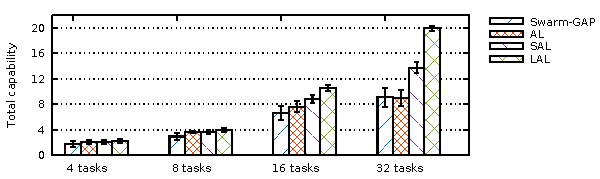
\includegraphics[scale=1.00]{total_capability.pdf}
		\caption{Total reward of each method for different scenarios with stimulus 0.6}
		\label{grafico:total_capability}
	\end{center}
\end{figure}

\subsection{Makespan and quantity of completed tasks}

The quantity of completed tasks for each algorithm in each scenario is presented in Figure \ref{grafico:tarefasconcluidas}. 
The results presented in this figure are normalized by the number of tasks of each scenario. Figure \ref{grafico:ticks} shows the elapsed time (in ticks), normalized by the deadline associated to the mission. 
As it is possible to observe, using time efficiently, the \uavs\ can perform more tasks achieving greater total rewards.

%\input{graficos/graficos_completed_tasks}
\begin{figure}[h]
	\begin{center}
		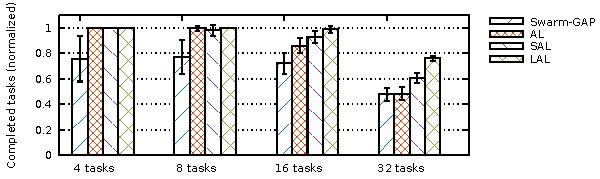
\includegraphics[scale=1.00]{completed_tasks.pdf}
		\caption{Completed tasks of each method for different scenarios with stimulus 0.6}
		\label{grafico:tarefasconcluidas}
	\end{center}
\end{figure}


%\input{graficos/graficos_ticks}
\begin{figure}[h]
	\begin{center}
		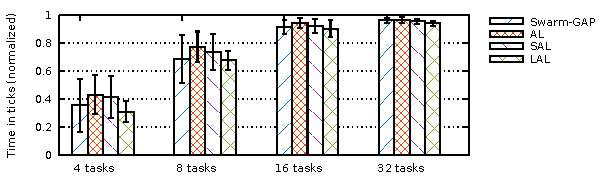
\includegraphics[scale=1.00]{makespan.pdf}
		\caption{Makespan of each method for different scenarios with stimulus 0.6}
		\label{grafico:ticks}
	\end{center}
\end{figure}

In scenarios with 4 and 8 tasks, in which there is enough time (extended or relaxed deadline) for the UAVs carrying out all the tasks (the whole mission), the Swarm-GAP algorithm results in \uavs\ not using all the available resources. In these cases they have used only 35.59\% and 68.81\% of the time. Moreover, more than 22\% of the tasks were not performed in these two scenarios. The slack time (65\% and 32\%, respectively, in scenarios with 4 and 8 tasks) could have been used to perform other tasks. On the other hand, using Allocation Loop (AL) method allowed 100\% and 99\% of the tasks to be performed. This was possible because while a \uav\ still has resources, it may select more tasks to perform in this method.

When the algorithms with Sorting and Allocation Loop (SAL), and Limit and Allocation Loop (LAL) were used, the \uavs\ have also performed all tasks in scenarios with 4 and 8 tasks. However, they took less time than the AL. The LAL, for instance, improves the elapsed time by 27\% and 12\% compared to AL in the scenarios with 4 and 8 tasks, respectively.

In scenarios with 16 and 32 tasks, i.e., those in which there are more tasks to be performed, the use of the SAL algorithm causes more tasks to be performed, in comparison to Swarm-GAP and AL, without increasing the elapsed time. For instance, in the scenario with 16 tasks, the use of SAL increased the amount of completed tasks by 28.8\% compared to Swarm-GAP. The LAL method improves this performance even further. 
In the scenario with 16 tasks, it happened simulation runs in which the UAVs have performed all tasks when using the LAL algorithm. Furthermore, in the scenario with 32 tasks, LAL increased the completed tasks by 59\%, whereas still reducing the elapsed time by 2.09\% compared to Swarm-GAP.

\subsection{Quality of completed tasks}

The average quality of the completed tasks in each scenario is shown in Figure \ref{grafico:qualidade}. The quality metric was normalized in relation to the number of completed tasks. The higher the quality of the tasks performed by the agents, the greater the total reward. For this measure, the LAL algorithm also shown the best results.

%\input{graficos/graficos_quality}
\begin{figure}[h!]
	\begin{center}
		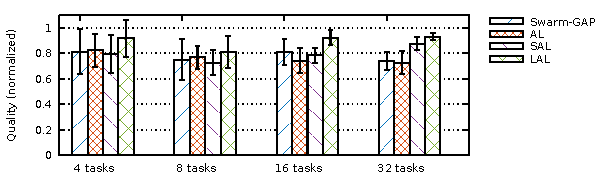
\includegraphics[scale=1.00]{quality.pdf}
		\caption{Quality of each method for different scenarios with stimulus 0.6}
		\label{grafico:qualidade}
	\end{center}
\end{figure}

In the scenarios with 4 and 8 tasks, the methods Swarm-GAP, AL, and SAL presented similar results in the quality of the completed tasks. However, Swarm-GAP outperformed SAL, but only in about 3\%. LAL increased by 12.74\% and 8.3\% the quality of the completed tasks in the scenario with 4 and 8 tasks, respectively, compared to the Swarm-GAP algorithm. 

In the scenario with 16 tasks, SAL still has a slightly lower result than Swarm-GAP (-3.2\%). However, when there are more tasks, such as in the scenario with 32 tasks, SAL improved the quality by 17.86\% compared to the Swarm-GAP. In the scenarios with 16 and 32 tasks, LAL presents an improvement of 13.92\% and 25.6\% compared to the Swarm-GAP, respectively. This pattern of quality improvement can also be observed in the other experiments 
with 64 and 96 tasks (see Table \ref{table:allresults6or9uavs}).

\subsection{Number of exchanged messages}

Figure \ref{grafico:trocamensagens} shows the number of exchanged messages for each algorithm in each scenario.
It is possible to notice that this number is nearly constant in the Swarm-GAP, AL and SAL, while in the LAL method the number of exchanged messages increases linearly with the amount of completed tasks. 
The behavior of  the three first algorithms is due to the fact that in these algorithms the number of the tokens that are sent relates more to the amount of agents than to the number of performed tasks.

%\input{graficos/graficos_msg}
\begin{figure}[h!]
	\begin{center}
		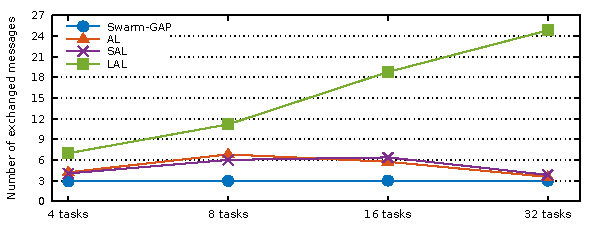
\includegraphics[scale=1.00]{exchanged_messages.pdf}
		\caption{Total number of exchanged messages of each method for different scenarios  with stimulus 0.6}
		\label{grafico:trocamensagens}
	\end{center}
\end{figure}

Using Swarm-GAP, each UAV receives the token at most once. When the UAV does not receive it, this means that all tasks were already selected before the token arrives to this given UAV. Anyway, when there is a given number of agents, for example three, the token is sent three times and then it is discarded. For AL and SAL, each \uav\ can receive the token more than once. On average, each \uav\ receives approximately one to two times the token.
Due to LAL's limitation of choosing at most one task at a time that the \uav\ receives the token, 
the number of exchanged messages is about the same number of performed tasks.

Despite the higher number of exchanged messages in the LAL algorithm, the quantity of completed tasks improved and the elapsed time decreased. Hence, the LAL algorithm enables \uavs\ to spend less time in the execution of each task, i.e., the cost to carry out the tasks decreases.

In order to investigate if this increase in the number of exchanged messages is rewarded by the quantity of completed tasks, Figure \ref{grafico:custoportarefa} presents the average cost to perform each task, considering also the number of exchanged messages. 
Then, the cost was computed by $avgcost = (t + em) / ct$, where ($t$) is the elapsed time, ($em$) is number of exchanged messages and ($ct$) is the amount of completed tasks.

%\input{graficos/graficos_custo}
\begin{figure}[h!]
	\begin{center}
		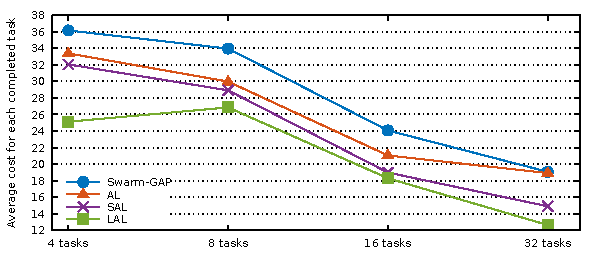
\includegraphics[scale=1.00]{avgcost.pdf}
		\caption{Average cost of the completed tasks (considering number of exchanged messages) of each method for different scenarios  with stimulus 0.6}
		\label{grafico:custoportarefa}
	\end{center}
\end{figure}

Even assuming that the amount of exchanged messages is also considered in the cost of executing the tasks, the LAL algorithm still reduces it compared to Swarm-GAP, by 30.48\%, 20.95\%, 24\% and 33.73\%, respectively for the scenarios with 4, 8, 16 and 32 tasks. 
 

\subsection{Algorithm's Runtime} \label{sec:runtime}

The scenarios \ref{case:32tasks}, \ref{case:64tasks} and \ref{case:96tasks}, which are composed of 32, 64, and 96 tasks, respectively, are used to illustrate the runtime results for the proposed algorithms.
The amount of \uavs\ in these scenarios is varied, and the number of tasks is greater. The runtime was measured in seconds, using the NetLogo profiler extension. 

The results of 30 runs (mean and standard deviation) of these scenarios, with all considered metrics (see Section \ref{sec:experimental_result}), can be seen in the Tables \ref{table:allresults3uavs} and \ref{table:allresults6or9uavs}. 
Here, the runtime analysis of each algorithm in different scenarios is highlighted in the Table \ref{table:runtime}.
This table shows the mean total runtime in seconds, 
the number of times the algorithm was executed and the mean runtime of each execution.
It is worth to notice that the number of times the algorithm was executed is the same of the number of exchanged messages.

\begin{table}[ht]
	\small
	\fontsize{8}{8}\selectfont
	\centering
	\caption{Runtime analysis of each method (in seconds) in different scenarios}
	\label{table:runtime}
	
	\begin{tabular}{clrrrr} \hline
		Scenario   &                               & Swarm-GAP &  AL     & SAL     & LAL    \\ \hline 
		32 tasks   & Total runtime (mean) in sec.  & 2.9778 & 3.2434 & 4.0268 & 10.9934 \\ 
		3 UAVs     & Execution times (mean)        & 3.0000 & 3.5333 & 3.8333 & 24.8000 \\ 
		           & Seconds per run               & 0.9926 & 0.9179 & 1.0504 & 0.4432  \\ [1ex]
		64 tasks   & Total runtime (mean) in sec.  & 7.2348 & 10.7935 & 9.7962 & 31.9513 \\ 
		6 UAVs     & Execution times (mean)        & 6.0000 & 6.5333  & 6.6333 & 44.0000 \\ 
				   & Seconds per run               & 1.2058 & 1.6520  & 1.4768 & 0.7261  \\ [1ex]
		96 tasks   & Total runtime (mean) in sec.  & 9.0990  & 13.1253 & 12.2062 & 50.5544 \\ 
		9 UAVs     & Execution times (mean)        & 9.0000  & 9.8667  & 9.7000  & 51.5000 \\ 
		           & Seconds per run               & 1.0110  & 1.3302  & 1.2583  & 0.9816  \\ [1ex] \hline 
	\end{tabular}
\end{table} 

The total runtime for AL and SAL are almost the same for each scenario. This suggests that sorting the tasks in SAL algorithm has not a great impact in the runtime. 
The AL and SAL results are close to Swarm-GAP in the scenario with 32 tasks. 
However, in the scenarios with 64 and 96 tasks, the availability check, that avoids the token remain in the network forever, impacts the runtime due to the greater number of tasks. 
For instance, the AL total runtime increases by 44.24\% compared to Swarm-GAP in the scenario with 96 tasks.

On the other hand, the LAL increases the total runtime for all scenarios compared to the others algorithms.
Due to the limit to select tasks, the LAL algorithm is executed more times causing the total runtime to increase. 
For example, in the scenario with 96 tasks, the LAL algorithm was executed on average 51.5 times -- that is the same number of exchanged messages. 
Although the LAL presented a high total runtime, each \uav\ took 0.9816 seconds, on average, to execute the algorithm each time it received the token in this scenario with 96 tasks.

\subsection{Discussions} \label{sec:discussion}
This section aims to identify the main aspects found during the replications done and to analyze all obtained results (see Section \ref{sec:findings}), identifying its implications for practice (see Section \ref{sec:implications}), characterizing the threats to the study validity (see Section \ref{sec:threats}), listing the main existing limitations in this work done and the opportunities to perform further investigations based on this one (see Section \ref{sec:limitations}).

\subsection{Scalability analysis} \label{sec:scalability}
In order to test the scalability of the proposed solutions, two new experimental scenarios were created. 
They have a very large number of agents and tasks (100 \uavs\ and 500 tasks) and differ from each other by the missions' deadline. These two additional scenarios are described as follows:

\begin{enumerate}
	\setcounter{enumi}{6}
	\item 100 \uavs; 500 tasks; 300 ticks as deadline; 750 x 750 px area size. \label{case:500tasks300deadline}
	\item 100 \uavs; 500 tasks; 1000 ticks as deadline; 750 x 750 px area size. \label{case:500tasks1000deadline}
\end{enumerate}

It is worth mentioning that the quantities used in these scenarios extrapolate those that would be expected in a real situation. However, the intention here is to stress these numbers to discuss scalability. 
The results (total reward, makespan, quantity and quality of completed tasks and number of exchanged messages) of 30 runs are shown in Table \ref{table:500tasks}.

\begin{table}%[t]
	\small
	\fontsize{6}{6}\selectfont
	\centering
	\caption{Total reward, makespan, quantity and quality of completed tasks and number of exchanged messages of 30 runs of each algorithm in scenarios with 100 \uavs\ and 500 tasks}
	\label{table:500tasks}
	
	\begin{tabular}{rrrrr} \hline
		& Swarm-GAP
		& AL
		& SAL
		& LAL \\ \hline 
		
		& Mean (St.Dev.) & Mean (St.Dev.)  & Mean (St.Dev.)  & Mean (St.Dev.)  \\ [1ex]
		
		\multicolumn{5}{l}{\textbf{100 UAVs and 500 tasks in area of 750x750 pixels with deadline of 300 ticks}} \\
		Total reward           &  162.0141  ($\pm$6.5974) &  162.9333  ($\pm$7.0324)   &  339.2015  ($\pm$7.5146)  &  240.956   ($\pm$3.6869)   \\
		Elapsed time (norm)    &  0.9979    ($\pm$0.0020) &  0.9978    ($\pm$0.0020)   &  0.9908    ($\pm$0.0029)  &  0.9992    ($\pm$0.0023)   \\ 
		Comp. tasks (norm)     &  0.4063    ($\pm$0.0141) &  0.4090    ($\pm$0.0161)   &  0.7269    ($\pm$0.0159)  &  0.5022    ($\pm$0.0075)   \\ 
		Quality (norm)         &  0.7789    ($\pm$0.0234) &  0.7736    ($\pm$0.0190)   &  0.9638    ($\pm$0.0085)  &  0.9707    ($\pm$0.0078)   \\ 
		%Idle UAVs              &  0.0000    ($\pm$0.0000) &  0.0000    ($\pm$0.0000)   &  0.4333    ($\pm$0.5683)  &  0.0000    ($\pm$0.0000)   \\ 
		Sending token          &  100       ($\pm$0.0000) &  103.4667  ($\pm$1.9070)   &  104.5333  ($\pm$1.8889)  &  298.1333  ($\pm$2.5695)   \\ 
		%Cost = (t + me) / ct   & 1.9660                  &  1.9697                   &  1.1055                  &  2.3811                   \\ 
		%Total Runtime (sec)    & 335.1766   ($\pm$92.466) &  550.796   ($\pm$261.7752) &  1164.9918 ($\pm$343.6324) &  2163.343 ($\pm$287.6923)  \\ 
		[1ex]	\hline
		
		\multicolumn{5}{l}{\textbf{100 UAVs and 500 tasks in area of 750x750 pixels with deadline of 1000 ticks}} \\
		Total reward           &  227.1356  ($\pm$8.4193)    &  230.5901  ($\pm$9.4936) &  435.3937 ($\pm$5.3410)    &  461.5992  ($\pm$2.0479)  \\
		Comp. tasks (norm)     &  0.7295    ($\pm$0.0213)    &  0.7420    ($\pm$0.0230) &  1.0000   ($\pm$0.0000)    &  1.0000    ($\pm$0.0000) \\ 
		Elapsed time (norm)    &  0.9983    ($\pm$8.0E-4)    &  0.9982    ($\pm$8.0E-4) &  0.9925   ($\pm$0.0028)    &  0.9856    ($\pm$0.0123)  \\ 
		Quality (norm)         &  0.7960    ($\pm$0.0173)    &  0.7902    ($\pm$0.0154) &  0.9650   ($\pm$0.0138)    &  0.9778    ($\pm$0.0058) \\ 
		%Idle UAVs              &  0.0000    ($\pm$0.0000)    &  0.0000    ($\pm$0.0000) &  38.7333  ($\pm$2.6773)    &  0.0000    ($\pm$0.0000)   \\ 
		Sending token          &  100       ($\pm$0.0000)    &  110.1667  ($\pm$2.6141) &  65.7667  ($\pm$4.2966)    &  526.1667  ($\pm$12.3821)  \\ 
		%Cost = (t + me) / ct   &  3.0111                    & 2.9875                  &  2.1165                   &  3.0235                   \\ 
		%Total Runtime (sec)    &  244.3903  ($\pm$30.1872)   & 356.2328   ($\pm$25.864) &  404.3574 ($\pm$343.8118)  &  2879.1853 ($\pm$567.0917)  \\ 
		[1ex]	\hline
	\end{tabular}
\end{table} 

The AL algorithm presented similar results to Swarm-GAP, in both scenarios (\ref{case:500tasks300deadline} and \ref{case:500tasks1000deadline}).
SAL had an increase of around 100\% in the total reward, compared to Swarm-GAP, in both scenarios.
LAL also outperformed Swarm-GAP in both scenarios. 
The total reward had an improvement of 48.72\% and 103.22\% when LAL is used, compared to Swarm-GAP, respectively in scenarios \ref{case:500tasks300deadline} and \ref{case:500tasks1000deadline}.

Although the LAL method presents the best results in most of the performed experiments, it was overcome by SAL in scenario \ref{case:500tasks300deadline}.
Due to the limit of selection imposed by the LAL, each \uav\ can select no more than 3 tasks in total. This is because the deadline is 300 ticks and there are 100 \uavs\ (at each tick one \uav\ receives the token). Thus, always less than 300 tasks will be performed, even if there are 500 tasks to be performed.
On the other hand, in the scenario \ref{case:500tasks1000deadline}, in which there is a large time window to the \uavs\ perform the tasks (1000 ticks of deadline), LAL is the best in terms of total reward.

% Colocar na tabela: seconds per run??


